\chapter{Observace, měření a reprezentace}
K pozorování meteorů a jejich záznamu se v současnosti používají tři přístupy: fotografické snímky, videozáznamy a radarová měření.

Ve všech třech přístupech je cílem sledovat a zaznamenávat celou oblohu nebo alespoň její velkou část. Například u fotografického přístupu se používá rybí oko \cite{ceplecha} -- čočka nebo objektiv, který je schopný zobrazit celou oblohu na jeden snímek. Cenou za takto širokoúhlý snímek je velké zkreslení obrazu, to lze ale pro účely měření matematicky odstranit \cite{ceplecha}.

\todo{Radarová měření dle \cite{radiosurvey}}

Fotografické snímky a videozáznamy jsou z hlediska měření velmi blízké: Videozáznam je v principu pouze série fotografií, v minulém století se ale využívalo spíše opačného přístupu, kdy se několik fotografických záběrů zaznamenalo na jeden snímek \cite{ceplecha}. Oba přístupy tedy dávají průběh polohy (a případně i luminosity) meteoru v čase. Konkrétně pro metody identifikace meteorických rojů potřebujeme právě dráhu (polohu) a rychlost meteoru \cite{ceplecha}, abychom zjistili orbitální dráhu meteoroidu. Důkladněji se zpracování fotografických snímků budeme věnovat v sekci \ref{sec:foto}.

\section{Elementy dráhy}
Orbitální dráhy jsou v prvním přiblížení elipsy, které jsou nakloněné v prostoru. Jedním z ohniskových bodů je vždy těžiště (Sluneční) soustavy, pro určení dráhy tedy stačí 5 parametrů \cite{astro}.

\medskip

Dva z parametrů popisují tvar elispy; její velikost a excentricitu \cite{astro}. \textit{Excentricita} $e$ náleží do intervalu $\left[0,1\right)$,\footnote{Excentricita může být také $=1$ pro parabolické a $>1$ pro hyperbolické dráhy. \ask{Otevřené, předpokládám, ignorujeme, protože by patřily do sporadického pozadí automaticky (nemají mateřský objekt ve Sluneční soustavě).}} a udává, jak blízká kružnici tato dráha je (viz obrázek \ref{img:excentricity}).

\todo{Ilustrace excentricit}

Pro určení velikosti používáme buďto \textit{délku hlavní poloosy} $a$ nebo \textit{vzdálenost perihelia} $q$ (efektivně vzdálenost okraje elipsy od ohniska). Jejich vztah ilustruje obrázek \ref{img:elipsa} a mezi oběma lze převádět pomocí rovnice \cite{ceplecha}
$$
    q=a(1-e)\text{.}
$$

\todo{Obrázek vztahu mezi $a$ a $q$}

\smallskip

Zbylé tři parametry určují natočení elipsy v prostoru. Jedná se o obdobu Eulerových úhlů, jsou ovšem definované vůči Slunci a ekliptice. Tyto úhly jsou znázorněny v obrázku \ref{img:elementy} a slovně se jedná o
\begin{itemize}
    \item \textit{inklinaci} $i$, která udává úhel mezi rovinou ekliptiky a rovinou elipsy \cite{astro},
    \item \textit{délku vzestupného uzlu} $\Omega$, která udává heliocentrickou ekliptikální délku bodu, ve kterém dráha protíná rovinu ekliptiky při průletu z jihu (tzv. \textit{vzestupný uzel}, \NorthNode) \cite{astro}, a
    \item \textit{argument perihelia} $\omega$, úhel, ve kterém se nachází perihelium, měřený od úsečky spojující Slunce a vzestupný uzel \cite{astro}.
\end{itemize}
Tyto úhly se aplikují jako rotace na rovinu ekliptiky s počátkem ve středu Slunce.

\begin{figure}[ht]
    \centering
    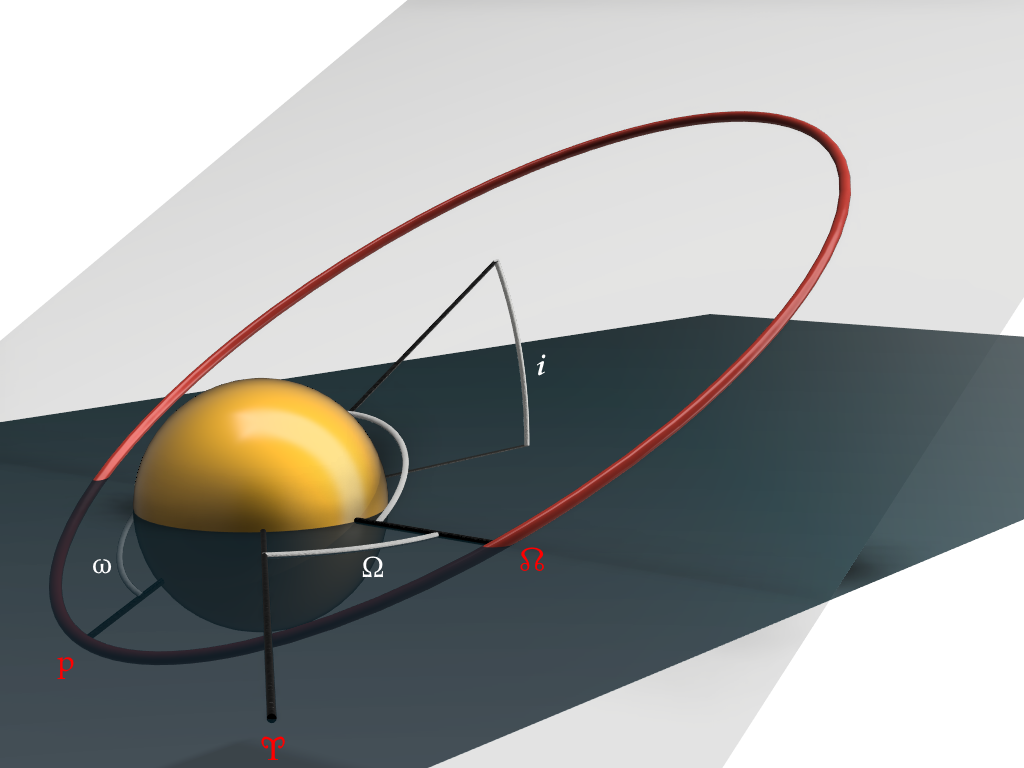
\includegraphics[width=0.8\linewidth]{img/orbit-elements-marked.png}
    \caption{Ilustrace významu elementů dráhy $i$, $\Omega$ a $\omega$ \cite{astro}}
    \label{img:elementy}
\end{figure}

\medskip

Na takto definované dráze se ještě můžeme setkat se souřadnicí zvanou \textit{pravá anomálie} $\nu$. Ta již nespecifikuje dráhu, nýbrž polohu objektu na své dráze, a v meteodách identifikace meteorických rojů nevystupuje. Udává se jako úhel měřený od spojnice Slunce a perihelia ke spojnici Slunce a objektu \cite{astro}.

\section{Fotografická měření\label{sec:foto}}
Úkolem astrometrických měření meteorů je zjistit elementy dráhy meteoroidu před tím, než se setkal s atmosférou Země. Vše ale začíná na fotografii nebo videozáznamu průletu meteoru atmosférou.

Budeme popisovat techniku měření používanou pro fotografická měření, kde máme fotoaparát s rybím okem pro zachycení celé oblohy a clonou, která s pevnou periodou (několikrát za vteřinu) zakrývá detektor nebo fotografický film, čímž zachytí časovou závislost pohybu meteoru. \todo{Bude-li obrázek, přidat a popsat.} Pro video je postup prakticky identický, hůře se ale ilustruje.

\medskip

Mějme tedy stanici \textbf{A} ležící na zeměpisné šířce $\varphi_\mathbf{A}$ a zeměpisné délce $\lambda_\mathbf{A}$, kde je umístěn fotoaparát s rybím okem a periodickou clonou tak, že zenit (kolmice k zemskému geoidu) leží uprostřed snímku, a přesné hodiny pro zaznamenání času měření. Fotoaparát v průběhu noci pořídí velké množství snímků a ke každému snímku umíme přiřadit přesný čas. Stejně tak mějme dále stanici \textbf{B}.

\note{Přidat vysvětlení, proč se pracuje s protínáním rovin, a ne prostě triangulací polohy.}

\smallskip

%#region Kroky (1)-(3): Měření kartézských souřadnic, převod na obzorníkové souřadnice, převod na rovníkové souřadnice II. druhu
Prvním krokem při zachycení meteoru je získat z fotografie jeho polohu v obzorníkové soustavě. K tomu nejprve snímek zkalibrujeme.

Začneme zavedením kartézských souřadnic na snímku s počátkem ve středu fotografie, který by měl být polohou zenitu. Přepočet z kartézských souřadnic $x,\,y$ na obzorníkové souřadnice $A,\,z$ provedeme pomocí vzorců \cite{ceplecha}
\begin{eqnarray}
    \begin{aligned}
        \tan{A-A_0}&=\frac{y-y_0}{x-x_0}\\
        z&=U+V\cdot r+S\cdot e^{D\cdot r}\text{, kde}
    \end{aligned}\label{eqn:lsqr}\\
    r^2=(x-x_0)^2+(y-y_0)^2\text{.}
\end{eqnarray}
Ve vzorcích \eqref{eqn:lsqr} jsou proměnné $A_0,\,x_0,\,y_0,\,U,\,V,\,S$ a $D$ neznámé a jejich hodnoty zjistíme fitováním metodou nejmenších čtverců z poloh hvězd.

Na snímku identifikujeme hvězdy, z katalogu zjistíme jejich polohy a pomocí geografické polohy a času měření přepočteme polohy hvězd do obzorníkových souřadnic $A_{\ast i},\,z_{\ast i}$. Na snímku také odměříme kartézkské souřadnice těchto hvězd $x_{\ast i},\,y_{\ast i}$. Páry souřadnic poté použijeme pro zjištění neznámých proměnných metodou nejmenších čtverců (detailně viz \cite[223--224]{ceplecha}).

S kompletními převodními vztahy \eqref{eqn:lsqr} převedeme jednotlivé otisky meteoru na jednom snímku z odměřených kartézských poloh $x_i,\,y_i$ na obzorníkové $A_i,\,z_i$. Ty následně přepočteme do rovníkových souřadnic {\uppercase\expandafter{\romannumeral 2\relax}}. druhu; za použití času měření $\vartheta_i$ a geografické polohy stanice $\varphi_\mathbf{A},\,\lambda_\mathbf{A}$ získáme deklinaci $\delta_i$ a rektascenzi $\alpha_i$ \cite{ceplecha}.
%#endregion

\smallskip

%#region Kroky (4)-(7): Nalezení střední roviny otisků ze stanice A
Z jednotlivých souřadnic $\delta_i,\,\alpha_i$ zadefinujeme složky
\begin{equation}
    \begin{aligned}
        \xi_i&=\cos{\delta_i}\cos{\alpha_i}\\
        \eta_i&=\cos{\delta_i}\sin{\alpha_i}\\
        \zeta_i&=\sin{\delta_i}
    \end{aligned}
\end{equation}
jednotkových vektorů
$$
\vec{\rho}_i=\begin{pmatrix}
    \xi_i\\\eta_i\\\zeta_i
\end{pmatrix}\text{,}
$$
které ukazují do směru jednotlivých otisků meteoru relativně vůči poloze stanice. V ideálním případě by všechny vektory $\left\{\vec{\rho}_i\right\}$ ležely v rovině, při reálných měřeních se ale od jisté střední roviny mírně odchylují. Zavedeme tedy (jednotkový) vektor $\vec{n}_\mathbf{A}$ jako normálový vektor definující tuto střední rovinu podmínkou, aby byl co nejvíce kolmý na $\vec{\rho}_i$, resp. přesněji jako jednotkový vektor $\vec{m}\in S_3(1)$ takový, že suma
$$
    \sum_{i}{\left( \vec{m}\cdot\vec{\rho_i} \right)^2}
$$
je minimální \cite{ceplecha} (suma by byla rovna nule, pokud by vektory $\vec{\rho}_i$ ležely v rovině).

Pro tuto podmínku lze analyticky nalézt jednoznačné řešení, kterým je \cite{ceplecha}
\begin{equation}
    \begin{aligned}
        \vec{n}^\prime=\begin{pmatrix}
            \left( \sum_{i}{\xi_i\eta_i} \right)\left( \sum_{i}{\eta_i\zeta_i} \right)-\left( \sum_{i}{\eta_i^2} \right)\left( \sum_{i}{\xi_i\zeta_i} \right)\\
            \left( \sum_{i}{\xi_i\eta_i} \right)\left( \sum_{i}{\xi_i\zeta_i} \right)-\left( \sum_{i}{\xi_i^2} \right)\left( \sum_{i}{\eta_i\zeta_i} \right)\\
            \left( \sum_{i}{\xi_i^2} \right)\left( \sum_{i}{\eta_i^2} \right)-\left( \sum_{i}{\xi_i\eta_i} \right)^2
        \end{pmatrix}\text{.}
    \end{aligned}
\end{equation}
Normalizací pak získáme požadovaný jednotkový vektor
\begin{equation}
    \vec{n}_\mathbf{A}=\frac{\vec{n}^\prime}{\lVert \vec{n}^\prime \rVert }\text{.}
\end{equation}

\smallskip

K určení roviny potřebujeme kromě normálového vektoru také jeden bod, kterým je v našem případě pozorovací stanice. Její geografické souřadnice známe, potřebujeme ale přejít do souřadinic geocentrických, ve kterých budeme provádět dalších několik kroků.

Geocentrické souřadnice udávají vzorce \cite{ceplecha}
\begin{equation}
    \begin{aligned}
        X&=(R+h)\cos{\varphi^\prime}\cos{\vartheta}\\
        Y&=(R+h)\cos{\varphi^\prime}\sin{\vartheta}\\
        Z&=(R+h)\sin{\varphi^\prime}\text{,}
    \end{aligned}
    \label{eqn:geocentric}
\end{equation}
kde $h$ je nadmořská výška objektu, $\vartheta$ je místní hvězný čas, $R$ je poloměr Země v kilometrech korigovaný na tvar geoidu v zeměpisné šířce $\varphi$ daný vzorcem \cite{ceplecha}
\begin{equation}
    R=\sqrt{40\,680\,669{,}86\frac{1-0{,}013\,343\,955\,4 \sin^2{\varphi}}{1-0{,}006\,694\,385\,096 \sin^2{\varphi}}}
\end{equation}
a $\varphi^\prime$ je geocentrická zeměpisná šířka \cite{ceplecha}
\begin{equation}
    \begin{aligned}
        \varphi^\prime=\varphi&-0{,}192\,424\,086\,7^\circ \sin{2\varphi}\;+\\
        &+0{,}000\,323\,122^\circ \sin{4\varphi}\;-\\
        &-0{,}000\,000\,723\,5^\circ \sin{6\varphi}\text{.}
    \end{aligned}
\end{equation}

Provedeme-li skalární součin normálového vektoru $\vec{n}_\mathbf{A}$ s vektorem geocentrické polohy stanice $\vec{a}=\left(\begin{smallmatrix}
    X\\Y\\Z
\end{smallmatrix}\right)$, získáme vzdálenost
\begin{equation}
    d_\mathbf{A}=\vec{n}_\mathbf{A}\cdot\vec{a}
\end{equation}
roviny od středu Země \cite{ceplecha} a rovinu pak můžeme zapsat rovnicí \cite{ceplecha}
\begin{equation}
    \vec{n}_\mathbf{A}\cdot\vec{\rho}=d_\mathbf{A}\text{.}
    \label{eqn:photo:plane_a}
\end{equation}
%#endregion

\medskip

%#region Kroky (8)-(12): Protnutí rovin pro přesnou lokalizaci otisku, získat polární souřadnice
Stejný postup zopakujeme pro stanici \textbf{B} s geocentrickým polohovým vektorem $\vec{b}$, kde na konci získáme druhou rovinu s rovnicí
\begin{equation}
    \vec{n}_\mathbf{B}\cdot \vec{\rho}=d_\mathbf{B}\text{.}
    \label{eqn:photo:plane_b}
\end{equation}
Průsečnice těchto dvou rovin je přímka, po které uvažujeme, že se meteor skutečně pohyboval -- jakási střední trajektorie, s jejíž pomocí odstraňujeme nepřesnosti záznamového média a technik přepočtu. Tato přímka je navíc určená i se vzdáleností od středu Země podle vzorců \eqref{eqn:geocentric}, kterou jsme doposud neznali.

\smallskip

Geocentrickou polohu jednotlivých otisků meteoru zjistíme s pomocí ještě třetí roviny, kterou zavedeme pro každý otisk meteoru: Pro jednu z pozorovacích stanic, uvažujme například stanici \textbf{A}, definujeme rovinu takovou, že obsahuje polopřímku tvořenou stanicí \textbf{A} s polohovým vektorem $\vec{a}$ a vektorem $\vec{\rho}_i$ a je kolmá na rovinu definovanou normálovým vektorem $\vec{n}_\mathbf{A}$ (rovnicí \eqref{eqn:photo:plane_a}). Tuto rovinu můžeme opět reprezentovat normálovým vektorem \cite{ceplecha}
\begin{equation}
    \vec{n}_i=\vec{\rho}_i\times\vec{n}_\mathbf{A}
\end{equation}
a vzdáleností
\begin{equation}
    d_i=\vec{n}_i\cdot \vec{a}\text{.}
\end{equation}
Tuto rovinu také můžeme zapsat ve tvaru rovnice a protnutím této roviny s rovinami \eqref{eqn:photo:plane_a} a \eqref{eqn:photo:plane_b} nalezneme polohu otisku meteoru na jeho střední trajektorii \cite{ceplecha}:
\begin{equation}
    \tag{\ref{eqn:photo:plane_a}}
    \vec{n}_\mathbf{A}\cdot\vec{\rho}=d_\mathbf{A}
\end{equation}
\begin{equation}
    \tag{\ref{eqn:photo:plane_b}}
    \vec{n}_\mathbf{B}\cdot\vec{\rho}=d_\mathbf{B}
\end{equation}
\begin{equation}
    \vec{n}_i\cdot\vec{\rho}=d_i
\end{equation}

Vyřešením této soustavy rovnic získáme jednoznačně určený vektor $\vec{\rho}$, který si pro účely dalších výpočtů přeznačíme na $\vec{\rho}\equiv\vec{r}_i$. Vektor $\vec{r}_i$ již není jednotkovým vektorem, nýbrž udává geocentrickou polohu meteoru v bodě $i$-tého otisku. Z jeho složek dostaneme pomocí vzorců \eqref{eqn:geocentric} zpět polární souřadnice; geocentrickou šířku $\varphi^\prime_i$, hodinový úhel $\vartheta_i$ a vzdálenost $(R+h_i)=\lVert\vec{r}_i\rVert$.
%#endregion